Một chiếc thanh mảnh có độ dài $L$ và trọng lượng $P$ phân bố đều. Thả thanh vào một chất lỏng có trọng lượng riêng gấp $\gamma$ lần trọng lượng riêng của thanh (với $\gamma>1$), rồi nhấc một đầu thanh lên bằng một lực kéo $T$ theo phương thẳng đứng với độ lớn có thể điều chỉnh được sao cho thanh nằm cân bằng và nghiêng một góc $\alpha$ so với phương thẳng đứng sao cho $0^\circ<\alpha< 90^\circ$. 

%Gia tốc trọng trường là $g$. 

%\footnote{Thông thường, ở trái đất, gia tốc trọng trường là $g= \SI{9.81}{m/s^2} \approx \SI{10}{m/s^2}$. Số $10$ này chính là số 10 trong công thức liên hệ giữa trọng lượng $P$ và khối lượng $m$, tức là ta có thể viết $P=mg$ thay vì $P=10m$.}

\begin{center}
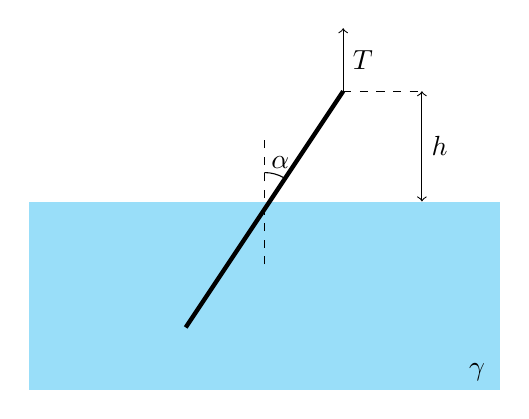
\begin{tikzpicture}[scale=1]
    \filldraw[color=white, fill=cyan!40] (-3,-1.2) rectangle (3,1.2);
    \draw[ultra thick] (-1,-0.4)--(1,2.6);
    \draw[dashed] (0,0.4)--(0,2);
    \draw (0.25,1.5) arc (60:90:0.5);
    \draw (0.2,1.5) node[above]{$\alpha$};
    \draw[dashed] (1,2.6)--(2,2.6);
    \draw[<->] (2,2.6)--(2,1.2);
    \draw (2,1.9) node[right]{$h$};
    \draw (2.7,-1.2) node[left,above]{$\gamma$};
    \draw[->] (1,2.6)--(1,3.4);
    \draw (1,3) node[right]{$\Vec{T}$};
\end{tikzpicture}
\end{center}

\begin{enumerate}[label=\textbf{\alph*,}]\itemsep0em
    \item Ban đầu $\alpha=\alpha_0$, thanh nằm cân bằng, độ cao đầu trên của thanh so với mặt nước là $h$. Tính $\alpha_0$ theo $\gamma$, $h$, $L$ và tìm điều kiện của $h$ theo $\gamma$, $L$ để thỏa mãn điều kiện $0^\circ < \alpha_0 < 90^\circ$.
    \item Dùng lực $T$ kéo chậm thanh khỏi mặt nước. Tìm công của lực kéo $T$ để kéo vật từ khi thanh nằm nghiêng góc $\alpha_0$ đến khi thanh vừa được kéo hoàn toàn ra khỏi mặt nước, biểu diễn kết quả theo $P$, $L$, $\gamma$ và $\alpha_0$.
\end{enumerate}


